\Introduction

Важной задачей изучения аттракторов внутренних волн с помощью численных методов является обеспечение возможности проводить численные эксперименты с геометрией, приближенной к геометрии реального дна океана. Выполнение этой задачи ускорило и удешевило бы процесс непостредственного поиска аттракторов внутренних волн в океане, и изучение влияния аттркаторов на турбулентные режимы. Метод спектральных элементов, который обеспечивает достаточную точность воспроизведения результатов эксперимента, ограничен в своей реализации сложностью геометрии расчетной области. В свою очередь, метод конечного объема позволяет работать со сложной геометрией, которая способна имитировать поверхность океанического дна, но стандартные реализации не обладают достаточной точностью. Кроме того, монохроматический источника возмущений может не описывать реальные внешние воздействия. Зачастую, при моделировании явлений, связанных с образованием аттракторов в реальных условиях, необходимо учитывать несколько приливных воздействий \cite{Garrett1972} и изменение стратификации.

Явление внутренних волн представляется собой нарушение состояние равновесия на границе раздела водяных слоев различной плотности. Выеденные из равновесия частицы жидкости начинают совершать колебания под действием силы тяжести и силы Архимеда.

Считается установленным, что впервые внутренние волны наблюдал американский ученый Франклин в восемнадцатом веке с помощью простой экспериментальной установки. Она представляла собой емкость, заполненную несмешивающимися жидкостями различной полости~\cite{Sudolski}. Однако в конце восемнадцатого века вблизи полуострова Таймыр произошло событие, которое заострило внимание научного сообщества на этом интересном явлении. В то время в этом районе пролегал маршрут исследовательского судна <<Фрам>>(Рис. \ref{fig:fram}) под руководством Фритьофа Нансена (Рис. \ref{fig:Nansen}).

Однажды во время штиля судно остановилось. Скорость его движения резко снизилась.  «чтобы пройти то небольшое расстояние, которое мы и на веслах прошли бы в полчаса или того меньше, «Фраму» понадобилась целая вахта», -- как писал сам Нансен. При этом исследователь отмечал, что вода на поверхности была пресной, потому как натекла с оттаявших ледников. А на глубине сравнимой с осадкой судна, резко становилась соленой. Позднее его записи послужили стимулом для теоретических исследований этого явления. В итоге было установлено, что почти вся энергия судового двигателя сдвигает не судно, а образует волны на поверхности раздела между слоями пресной и соленой воды. Это явление получило название <<мертвая вода>>.

Также существует еще одно свидетельство этого явления. Теплоход «Маршал Жуков» при проходе пролива Дарданеллы угодил в <<мертвую воду>> летом 1981 года. Уже в сентябре в отраслевой газете <<черноморец>> капитан-наставник Александр Косилов подробно описал как в течении четырех суток судно, держащее курс из Канады в Новороссийск, боролось с феноменом. Согласно комментариям руководителя аналитико-исследовательской группы управления инвестиций и проектов ОАО «Новошип», кандидата технических наук, профессора кафедры судовождения ГМУ им. адмирала Ф.Ф. Ушакова Юрия Пескова современные суда в значительной степени подвержены влиянию подобных явлений\cite{MorVest}. На то есть причины:

\begin{itemize}
    \item Экономия топлива вынуждает снижать скоростные режимы
    \item Борьба за уменьшение углекислых выбросов предписывает снижать мощность двигателя
\end{itemize}


\begin{figure}
    \centering
    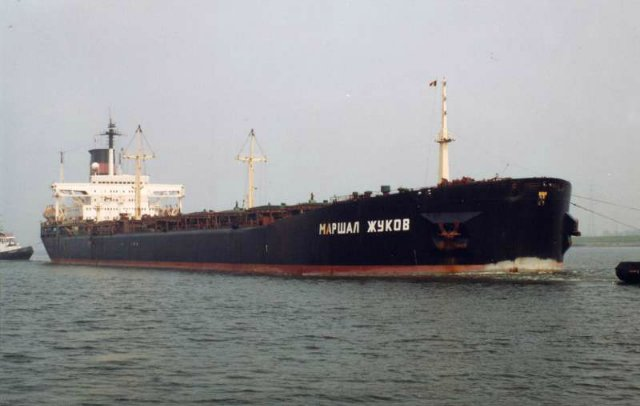
\includegraphics[scale=0.5]{Figs/marshl_jukov.jpg}
    \caption{Судно <<Маршал Жуков>>}
    \label{fig:jukov}
\end{figure}

И подобные явления, как оказалось, описывались и задолго до Франклина. В своей <<естественной истории>> Плиний Старший говорит о похожем явлении \cite{Plinii}. Позднее <<мертвая вода>> была воспроизведена в лабораторных условиях исследователями из франции \cite{deadWater}. Запись эксперимента доступна на видеохостинге youtube \cite{deadWaterVideo}.


Математически описать возникновение внутренних волн можно записав уравнение для сил, которые действуют на выведенную из равновесия частицу жидкости(Рис. \ref{fig:Forces}):

\begin{equation}
    m_b \vec{a}_b = \vec{P} + \vec{G}
\end{equation}
где $\vec{P}=\rho_w \vec{g} S \cdot h$ это сила Архимеда, $\rho_w$ плотность жидкости того слоя на котором находится частица, $\vec{g}$ -- ускорение свободного падения, $S$ -- площадь стороны частицы, $h$  -- глубина. $\vec{G} = \rho_b \vec{g} S \cdot h$,  $\rho_b$ -- плотность частицы жидкости.

В проекции на вертикальную ось:

\begin{equation}
    \frac{d^2 \xi}{dt^2} = \frac{(\rho_w-\rho_b)}{\rho_b}\cdot g
\end{equation}

Тут $\xi$ будет обозначать отклонение от положения равновесия $z_0$, тогда очевидно что плотность воды вокруг частицы и плотность частицы будет равна в положении равновесия при $\xi=0$ $\rho_w(z_0)=\rho_b$ тогда уравнение можно переписать:

\begin{equation}
    \frac{d^2 \xi}{dt^2} = \frac{\rho_w(z_0+\xi)-\rho_b}{\rho_b}\cdot g
    \label{eq:beg}
\end{equation}

Введем переобозначение, $z=z_0+\xi$ тогда правая часть уравнения запишется $$\frac{\rho_w(z_0+\xi)-\rho_b}{\rho_b}\cdot g = \frac{\rho_w(z)-\rho_w(z_0)}{\rho_w(z_0)}\cdot g = \frac{1}{\rho(z_0)} \frac{\rho_w(z)-\rho_w(z_0)}{z-z_0}\cdot(z-z_0) g$$

При достаточно малом $t$ отклонении от положения равновесия $z$ будет также мало, что дает нам возможность перейти к производной по $z$, а $\rho_w$ переобозначим как $\rho$ и окончательно запишем:

\begin{equation}
    \frac{d^2 \xi}{dt^2} =\frac{1}{\rho} \frac{d\rho}{z}\xi \cdot g
\end{equation}

Решение этого дифференциального уравнения ищется в виде периодической функции, это значит, что частица совершает колебания около своего положения равновесия:

\begin{equation}
    \xi(t)=A cos(\omega t + \phi)
\end{equation}

подставим выражения $\xi(t)$ в уравнение:

\begin{equation}
    \ddot{\xi} = - A \omega^2 cos(\omega t + \phi )
\end{equation}

или если выразить правую часть через $\xi$

\begin{equation}
    \ddot{\xi} = - \omega^2  \xi
    \label{eq:final}
\end{equation}

Подставим (\ref{eq:final}) в (\ref{eq:beg}):

\begin{equation}
    -\omega^2 \xi = \frac{1}{\rho_0}\cdot \frac{d \rho}{d z} \xi g
\end{equation}

Выразим частоту колебаний частицы:

\begin{equation}
    \omega(z) = N(z) = \sqrt{- \frac{g}{\rho_0}\cdot\frac{d \rho(z)}{dz}}
\end{equation}

Эта частота называется частота плавучести или Частота Брента — Вяйсяля. В океане она составляет величину порядка $10^{-3}$ $\frac{1}{\textup{с}}$ \cite{King2012}.

\begin{figure}
    \centering
    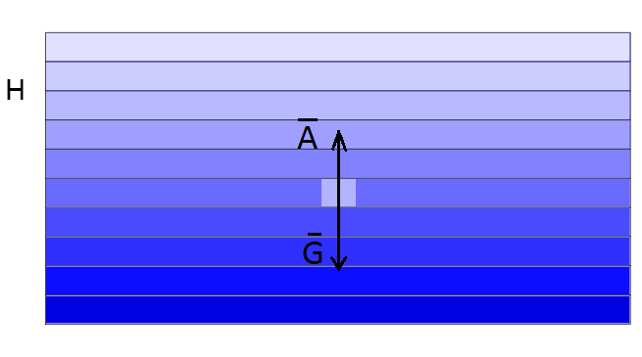
\includegraphics[scale=0.8]{Figs/Forces.png}
    \caption{Схематичное представление сил действующие на частицу выведенную из равновесия в стратифицированной жидкости, цветом показана плотность.}
    \label{fig:Forces}
\end{figure}

\begin{figure}
    \centering
    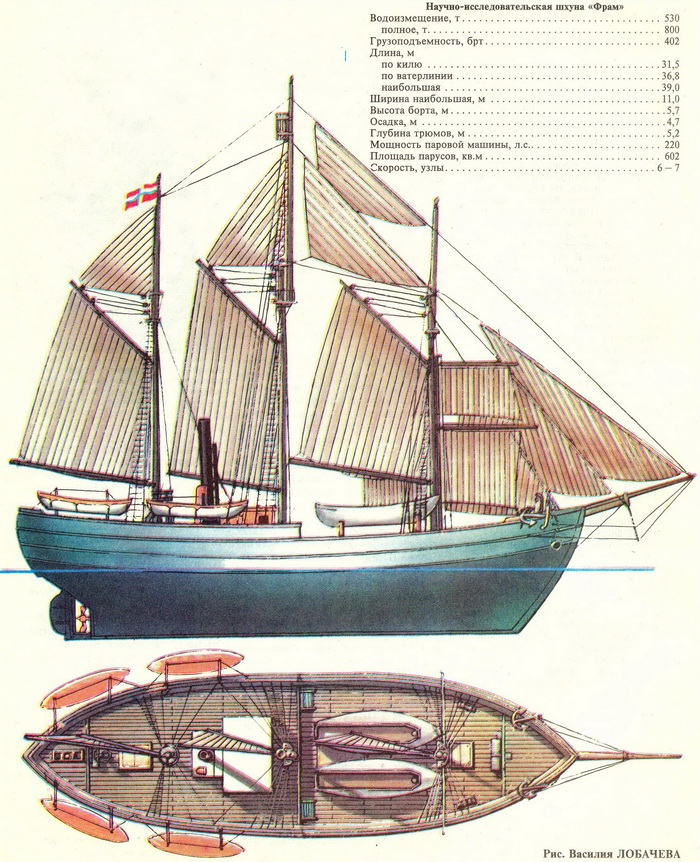
\includegraphics[width=1\textwidth]{Figs/FRAM.jpg}
    \caption{Исследовательское судно <<Фрам>>}
    \label{fig:fram}
\end{figure}

\begin{figure}
    \centering
    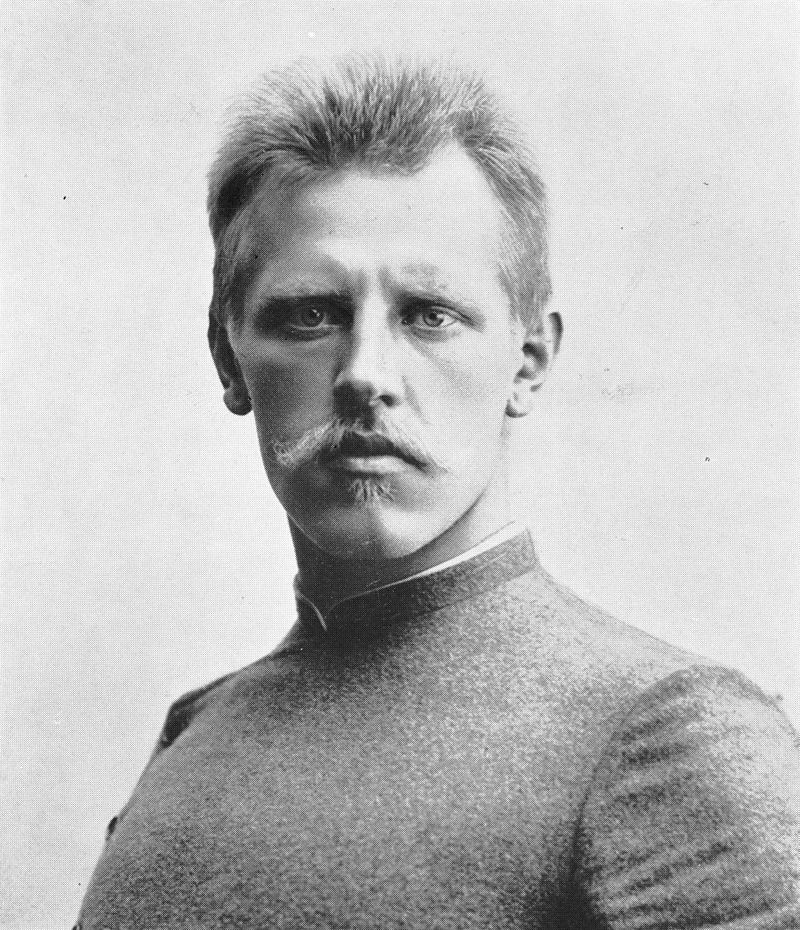
\includegraphics[scale=2.5]{Figs/800px-Fridtjof_Nansen.jpg}
    \caption{Фритьоф Ведель-Ярлсберг Нансен (1861-1930)}
    \label{fig:Nansen}
\end{figure}

\section{Обзор литературы}

Внутренние волны очень распространенное явление в океане. Существуют они благодаря перепадам плотности на разной глубине, сила плавучести играет роль восстанавливающей силы. Океаны являются одним из естественных примеров стратифицированных сред. Основные источники внутренних волн в океане это приливные эффекты, которые сопряжены с движением Земли относительно Солнца и Луны относительно Земли.

Внутренние волны активно взаимодействуют с другими океаническими структурами \cite{Rainville2006} и с неровностями океанического дна \cite{DAUXOIS1999}. Процессы перемещения внутренних волн их взаимодействия друг с другом и океаническими структурами различных масштабов образуют собой явление называемое энергетическим каскадом\cite{Garrett1972}. Энергетический каскад способствует поддержанию глобальной океанической циркуляции и перемешиванию\cite{Nikurashin2012,Munk1998}. Тем не менее, механизмы вносящие крупномасштабный приливный вклад в движение внутренних волн недостаточно понятны \cite{Ivey2008,Polzin1997} и каскадный процесс остается одной из фундаментальных проблем современной океанографии. Главным образом остаются вопросы связи крупномасштабных и мелкомасштабных явлений.

Одним из объяснений этой связи могут послужить аттракторы внутренних гравитационных волн. Это явление, при котором внутренние волны многократно отражаясь от поверхности океана, его дна и неровностей движутся по замкнутым орбитам. Возникновение такого явление возможно лишь в том случае, когда на дне океана имеются определенные комбинации геометрических неровностей. Аттракторы передают кинетическую энергию крупномасштабных эффектов, такие как приливы и внутренние волны большой длинны к мелкомасштабным явлениям волновой турбулентности и перемешиванию. Происходит это благодаря явлению фокусировки, в результате которого длинна внутренних волн уменьшается, но увеличивается амплитуда.

Возможность возникновения аттракторов в океане с реальной геометрией дна уже исследовалась\cite{Tang2010}. Например, топология северной части хребта Лусона имеет соответствующую геометрию. Эксперименты~\cite{ECHEVERRI2011} подтверждают возможность образования аттракторов внутренних волн. Кроме того при моделировании внутренних волн в условиях случайного разреза геометрии океанического дна, был сделан вывод, что с немалой вероятностью возможны возникновения аттракторов по одному на каждую сотню километров океанического дна \cite{Guo2015}. Тем не менее стоит отметить, что на данный момент нет свидетельств наблюдаемых волновых аттракторов. Возможно это связано с тем, что теоретические работы\cite{Guo2015} относятся к двумерному океану, но также существуют трехмерные конфигурации геометрий в которых возможны существования трехмерных волновых аттракторов\cite{Drijfhout2007,Manders2004}. Кроме того, в теоретическом представлении аттракторов внутренних волн не учитывается шероховатость поверхностей отражения. Однако надежность теоретических соображений о возможности существования трехмерных аттракторов была экспериментально проверена\cite{Hazewinkel2010}. Кроме того волновые явления в океане часто имеют целый спектр частот\cite{Garrett1972}, в то время как многочисленные эксперименты проводятся лишь с монохроматическим источником внутренних волн.

Предполагается, что аттракторы могут влиять не только на перемешивание, но и на движение мелких животных, явление седиментации и эрозию прибрежных конструкций.

Работы по фокусировке внутренних волн и образованию устойчивых аттракторов ведутся с конца двадцатого века. Первое теоретическое предсказание аттракторов было сделано Лео Маасом в 1995 году\cite{Maas1995}. Через два года последовали экспериментальные исследования этого явления, теоретические результаты были воспроизведены\cite{Maas1997}. Эффекты фокусировки характерны не только для стратифицированной жидкости, но и для вращающихся \cite{articleMaas2003,Veronis1970}. В дальнейшем теоретические основы явления были пересмотрены на основании данных эксперимента\cite{Lam2008}.

Вместе с развитием вычислительной техники развивались и инструменты численного моделирования физических явлений. Во втором десятилетии двадцать первого века стало возможным численное моделирование трехмерных аттракторов внутренних волн. Первая удачная попытка была предпринята с использованием метода спектральных элементов\cite{Brouzet2016,Brouzet_2016}. При сравнении с экспериментом ошибка численного моделирования составила не больше 10\%. Также была предпринята попытка моделирования аттрактора внутренних волн с помощью метода конечного объема\cite{Brouzet2014}. Количественно воспроизвести результаты, полученные с помощью метода спектральных элементов не удалось.
Традиционно для моделирования аттракторов применяются уравнения Навье-Стокса в приближении Буссинеска. Однако существует ряд работ, где вместо классического подхода используется квазигидродинамический\cite{ElizarBook}. Квазигидродинамические уравнения позволяют добиться большей точности\cite{Kraposhin20182} при моделировании методом конечного объема.

Результаты работы представляют собой интерес для приложений в океанологии, экологии, биологии, астрофизики и вращающихся технических систем. 

\paragraph{Цель работы} -- изучение явления бигармонического аттрактора, которое возникает при воздействии на стратифицированную жидкость двухчастотным волнопродуктором.  
С этой целбю были посталены следующие задачи \textbf{задачи}:

\begin{itemize}

  \item Нахождение интервала частот внешних воздействий, при которых возникает аттрактор внутренних волн.
  
  % Изучение интервалов частот внешних воздействий и других параметров, при которых происходит аккумуляция волновой энергии, в частности волновых аттракторов.

%    \item Нахождение частотных параметров приводящих к образованию аттракторов в резервуаре.
    
  % \item Обзор существующих методов моделирования аттракторов внутренних волн. Выявление их достоинств и недостатков.
    
  \item Реализация численных экспериментов с помощью двух подходов: спектрально-элементного и конечно-объемного.

  \item Разработка новой программы для моделирования аттракторов внутренних волн на основе квазигидродинамического подхода.
    
  \item Верификация результатов численного моделирования.

  \item Описание особенностей волновых режимов при бигармоническом воздействии и значительно отличающихся частотах воздействия и малых амплитудах.

  \item Описание особенностей волновых режимов при бигармоническом воздействии, близких частотах воздействия и малых амплитудах.
    
  \item Описание особенностей нелинейных волновых режимов при бигармоническом воздействии и близких частотах воздействия.

  \item Сравнение динамики средней кинетической энергии и пульсации кинетической энергии для монохроматического режима и различных бигармонических режимов.
    

    
\end{itemize}

\paragraph{Методы решения поставленных задач}

Для решения поставленых задач были использованы методы математического моделирования механики сплшных сред, такие как метод спектральных элементов и метд конечного объема. Для предсказания формы аттрактора внутренних волн использовался метод трассировки лучей. Для анализа данных использовался метод построения частотно-временных диаграмм при помощи быстрого преобразования Фурье.

\paragraph{Научная новизна работы} выражается в конкретных реузьтатах:
\begin{enumerate}[1.]
  \item Получены аналитические выражения для границ частотного интервала существования аттракторов внутренних волн.% конфигурации (1,1). 
    
  \item Получена геометрия течения, которая возникает в трапециевидном резервуаре, наполненном стратифицированной жидкостью при воздействии на жидкость внешними возмущениями с двумя различными частотами. 
    
  \item Проведён анализ результатов моделирования аттрактора внутренних волн при бигармоническом воздействии, полученных с помощью метода спектральных элементов. Для различных комбинаций возмущающих частот построен спектр, частотно-временная диаграмма и зависимость средней кинетической энергии от времени. 
    
  \item Реализован квазигидродинамический подход на базе метода конечного элемента. Проведено сопоставление результатов моделирования методов конечных объемов и методом спектральных элементов.
\end{enumerate}

\paragraph{Достоверность результатов}

Достоверность полученных результатов гарантируется строгой математической постановкой, верификацией и валидацией разработанного алгоритма для решения поставленной задачи.

% \paragraph{Объектом исследования} являются волновые режимы возникающие %в естественных условиях 
% при двух источниках внешних воздействий на стратифицированную жидкость в трапециевидном резервуаре.

% %Приложения включают в себя задачи океанологии, астрофизики и технических вращающихся систем при периодических воздействиях. 

% %\paragraph{В исследовании использованы следующие методы:}
% \begin{itemize}
%   \item [    В исследовании использованы \textbf{
% методы:}]
%   \item методы численного моделирования конечного объема;
%   \item метод спектральных элементов;
%   \item метод трассировки лучей;
%   \item Фурье анализ полученных результатов, в том числе по скользящему окну;
%   \item разложение по эмпирическим модам;
% \end{itemize}

% % В работе рассматриваются резервуары в форме трапеций различных конфигураций, заполненных стратифицированной жидкостью. Одна из стенок резервуара представляет собой волнопродуктор, который порождает внутренние волны в стратифицированной среде. Результаты разработки предоставляют возможность проводить моделирование аттракторов внутренних волн в условиях сложной геометрии и неортогональных сетках. 



\paragraph{Практическая значимость} 

Ранее эксперименты по исследованию бигармонических аттракторов, как численные так и натурные, не проводились. Теоретически, бигармонический аттрактор представляет собой новую устойчивую структуру, которая образуется в стратифицированной жидкости при воздействии на нее периодическим двухчастотным возмущением.

Положения и выводы диссертационного исследования могут быть использованы для подбора параметров  волнового аттрактора в лабораторных условиях или при численном моделировании. Среди возможных приложений результатов работы — задачи моделирования аттракторов внутренних волн на сложных геометриях, задачи моделирования течений со сложным спектром частотных воздействий на стратифицированную жидкость. Работа является первым шагом к моделированию течений, возникающих в условиях, приближенных к реальным океаническим, что позволит выяснить форму и вид природных аттракторов внутренних волн. Комбинация методов конечного объёма и квазигидродинамических уравнений позволила добиться существенного улучшения в точности моделирования и дала инструмент к  усложнению геометрии расчётной области. Разработанная программа может быть применена не только к задачам моделирования аттрактора, но и к другим задачам гидродинамики с дозвуковыми и трансзвуковыми скоростями.

\paragraph{На защиту выносятся следующие положения:}
\begin{itemize}

  \item Найдены аналитические выражения для границ диапазонов частот колебаний волнопродуктора, которые способны порождать аттракторы.

  \item Показано, что при значительном отличии частот внешних воздействий и малых амплитудах воздействий волновой режим представляет из себя совокупность независимо существующих волновых аттракторов.

  \item Показано, что при близких частотах внешних воздействий и малых амплитудах возникает режим с биениями, характерной особенностью которых является малая амплитуда пульсаций на убывающем склоне огибающей.

  \item Показано, что при близких частотах внешних воздействий и средних амплитудах возникают биения, на одном цикле которых успевает происходит переход к турбулентности через триадные резонансы, и реламинаризация.
    
  \item Обнаружено наличие фазового сдвига между биениями на волнопродукторе и биениями средней кинетической энергии во всем объеме.
    
%   \item 
%     Сравнение динамики средней кинетической энергии и пульсации кинетической энергии для монохроматического режима и различных бигармонических режимов указывает на то, что на убывающем склоне огибающей большая доля кинетической энергии переходит в бегущие волны по сравнению с возрастающей фазой.

  \item Разработана и верифицирована новая программа для моделирования аттракторов внутренних волн и в целом динамики стратифицированных сред.
    
%  \item Реализация численных экспериментов с помощью двух подходов: спектрально-элементного и конечно-объемного.

%  \item Проведена верификация результатов численного моделирования.
%    Проведение численных экспериментов различными методами.
    
%  \item Количественный анализ результатов численных экспериментов. 
    
%  \item Верификация разработанной программы.
    
\end{itemize}

\paragraph{Личный вклад автора}

Исследования, результаты которых выносятся на защиту, были получены лично соискателем. Соискатель аналитически нашел диапазон частот внешнего воздействия при которых образуется аттрактор внутренних волн. Соискатель подобрал параметры эксперемента, провел расчеты и проанализировал полученные данные. Также принимал непосредственное участие в разработке реализации квазигидродинамического подхода на базе открытого программного комлекса OpenFOAM. Научный руководитель И. Н. Сибгатуллин поставил первоначальную задачу и участввал в обсуждении результатов. 

\paragraph{Аппробация работы}

Материалы диссертации представлялись на различных конференциях, семинарах, как российсих так и международных:


\begin{itemize}
  \item Открытая международная конференция ИСП РАН им. В.П.Иванникова. 5-6 декабря 2019 г, г. Москва Главное здание Российской академии наук (устный доклад).
  \item Международная конференция «Суперкомпьютерные технологии математического моделирования» (СКТеММ’19), 19-21 июня 2019, г. Москва (устный доклад).
  \item 13th OpenFOAM Workshop, Shanghai, China, Китай, 24-29 июня 2018 (устный доклад).
  \item XXIII международная конференция «Нелинейные задачи теории гидродинамической устойчивости и турбулентность». 25 февраля - 4 марта 2018, Московская область, г. Звенигород (стендовый доклад).
  \item Рязанов Д.А. Открытая конференция ИСП РАН им. В.П. Иванникова. 30 ноября - 1 декабря 2017 г. Москва главное здание Российской академии наук (стендовый доклад).
\end{itemize}

\paragraph{Публикации}

По результатам диссертации опубликовано 12 научныйх работ, входящих в базы данных и системы цитирования РИНЦ, Scopus, Web of Science, 2 из них входят в Перечень рецензируемых научных изданий, рекомендованных Высшей раттестационной комиссией. Зарегестрирована программа для ЭВМ.

\paragraph{Сутрктура и объем диссертации}

% В ходе работ был разработан программный продукт, который подлежал государственной регистрации № 2018663951.
